\chapter{Load Testing}
We used Tsung~\cite{tsung} framework for load testing. We designed a \textit{generic workflow} which was able to capture the usual activities of a user while covering most, if not all, features of our website. We ran most of our tests on this generic workflow. Testing on the generic workflow gave us a rough idea on the overall performance of our website and possible bottlenecks. Later we created \textit{specific workflow} separating out the portions that we thought might be causing the greatest bottlenecks. We ran our tests on this specific workflow before and after optimization to verify that this was indeed the workflow that was causing the bottlenecks and that these have been remediated by the optimizations.
\section{Generic Workflow}\label{sec:generic-workflow}
In this workflow, at first a user logs in to the website. The user waits for a time between zero and two seconds, visits the games index page, and then waits again for a time between zero and one second. Then the user randomly visits a game page, waits for a time between zero and two seconds, comments on that game and then logs out. This concludes the first sessions of our workflow. 

In the second session, a user browses to the search page, searches for games by name, waits for a time between zero and one second, visits a random games page, waits for a time between zero and two seconds, searches for games by number of backgrounds, waits for a time between zero and two seconds, and visits a random game page. 

In the third session, a user browses to the gamers index page, waits between zero and one second, randomly gets a game, waits between zero and one second, browses to the genres page, waits between zero and one second, and finally browses to the companies page.

In the fourth session, a user browses to the signup page, waits for zero to three seconds, submits the form, waits for zero to one second, visits the games index page, waits for zero to one second, and finally likes/dislikes a random game.

\section{Specific Workflow}\label{sec:specific-workflow}

\begin{figure}
\centering
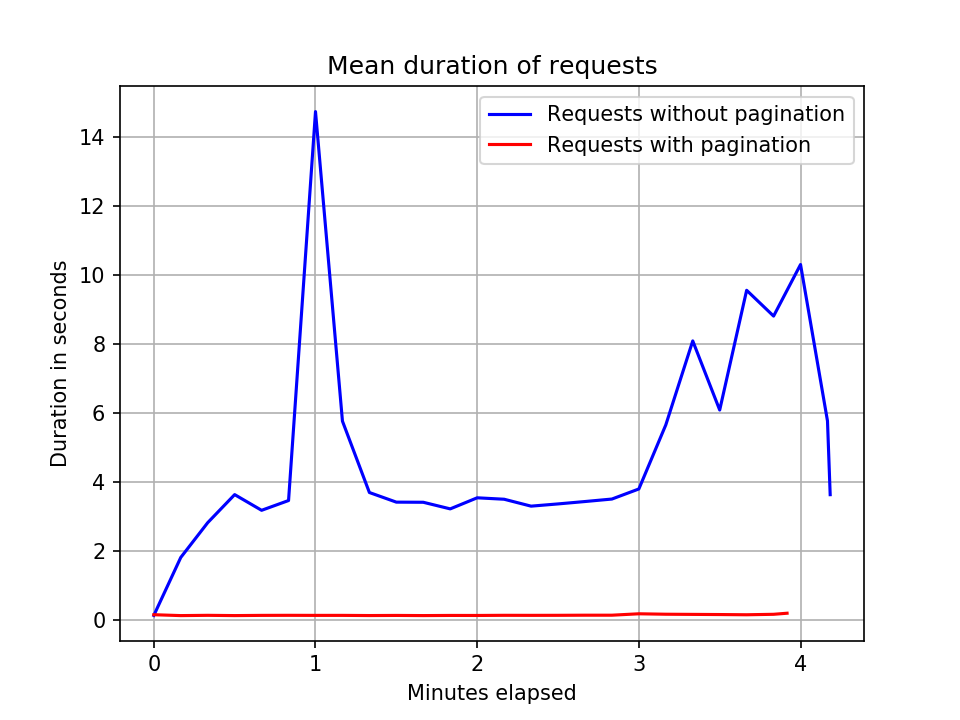
\includegraphics{images/tsung/request_mean_game_index_pagination.png}
\caption{Mean duration of pages before and after pagination for scenario in Section~\ref{sec:scenario-list-all-games}}\label{fig:effect-of-pagination-on-game-list}
\end{figure}
